\subsubsection{La funció printPersonsToTable()}

\paragraph{}
Aquesta funció, acaba de configurar els paràmetres necessaris per poder realitzar la cerca, la llença i en tracte la resposta.

En concret, configura els paràmetres \emph{inici} i \emph{context} i tot seguit, llença la crida asíncrona cap al SDK. Aquests paràmetres, ja han estat descrits en seccions anteriors de la memòria, però recordem que s'encarreguen de delimitar el primer resultat a retornar i a quina cerca es fa referència, en cas de trobar-se demanant més blocs de resultats a l'API de FamilySearch.

Si no es produeix cap error, l'API retornarà els primers quinze resultats i aquests es pintaran sobre una taula. En cas contrari, l'aplicació ensenyarà l'error a l'usuari tot indicant-ne el motiu de fallida.

\begin{lstlisting}[style=rawOwn,caption={Llençament de peticions contra el SDK i captura d'errors}]
client.getPersonSearch(params).then(function(searchResponse) {
    // Get persons and display id, name, birth date, death date
    ...
})
.catch(function(e) {
    // Display error
    ...
});
\end{lstlisting}

L'estructura de codi anterior, encarregada de llençar una petició al SDK i capturar possibles errors, és l'estàndard que segueixen totes les crides realitzades a la nostra aplicació web, que interactuen amb el SDK de FamilySearch.

La llista de resultats, que s'obté com a resultat d'una cerca, és mostra a la figura~\ref{fig:searchTableResults}.

\begin{figure}[h]
    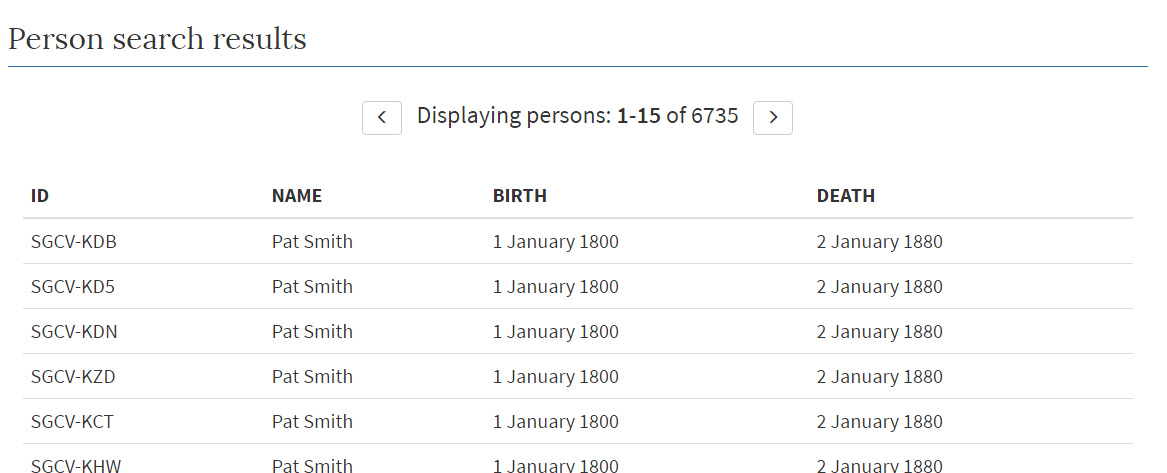
\includegraphics[width=\linewidth]{11/02_searchPersons/01_resultsTable}
    \centering
    \caption{Exemple de resultats d'una cerca a l'arbre familiar}\label{fig:searchTableResults}
\end{figure}

La gràcia de l'operació \emph{printPersonsToTable(pos)}, és que poden reutilitzar-la quan l'usuari vol navegar pels diferents blocs o pàgines de resultats, sense la necessitat de revalidar el formulari de cerca.

Quan el SDK retorna els resultats al controlador, aquest emmagatzema en variables globals, els paràmetres resultats totals, índex del primer resultat mostrat i context de la cerca.

Gràcies a aquestes variables, la funció es pot encarregar de configurar els paràmetres: posició d'inici i context, just abans de realitzar la cerca contra el SDK i per tant, pot ser reutilitzada amb facilitat, conjuntament a l'objecte \emph{params}, per demanar més blocs de resultats d'una cerca realitzada.

\begin{lstlisting}[style=rawOwn,caption={Actualització i utilització dels parametres \emph{count}, \emph{start} i \emph{context}}]
function printPersonsToTable(pos) {
    // Update start params
    params.start = pos;
    params.context = context;

    // Search with the defined parameters
    client.getPersonSearch(params).then(function(searchResponse) {
        // Get parameters
        count = searchResponse.getResultsCount();
        start = searchResponse.getIndex();
        context = searchResponse.getContext();
        ... // tractament dels resultats
    });
}
\end{lstlisting}
